\documentclass[12pt]{article}

\usepackage{sbc-template}

\usepackage{graphicx,url}

%\usepackage[brazil]{babel}   
\usepackage[latin1]{inputenc}  
\usepackage[utf8]{inputenc}  
\usepackage{verbatim}
\usepackage{listings}
\usepackage{xcolor}
\usepackage{indentfirst}
\usepackage{longtable}
\usepackage{lipsum} 

\definecolor{verde}{rgb}{0,0.5,0}

%para customizar o código (ver https://en.wikibooks.org/wiki/LaTeX/Source_Code_Listings)
\lstset{language=C, %defina a linguagem usada no trabalho
              belowcaptionskip=1\baselineskip,
                breaklines=true,
                frame=false,
                xleftmargin=\parindent,
                showstringspaces=false,
                basicstyle=\footnotesize\ttfamily,
                keywordstyle=\bfseries\color{green!40!black},
                commentstyle=\itshape\color{purple!40!black},
                identifierstyle=\color{blue},
                stringstyle=\color{orange},
                numbers=left,
            }

\sloppy

\title{Initial Report\\ ALOHA \\Distrubuted chat system}

\author{Alexandru Mihail Orlando, Darkhan Akhmediyev, Fiza Razzaq, \\ Lyubomir Vasilev, Sara Zain, Suhrita Kapilavayi}


\begin{document} 

\maketitle

\section{Project Description}

The aim of this project is to build a user friendly distributed chat system which allows two different clients (web and iOS) to communicate securely with one another in real time. It follows Client-Server Architecture based on socket programming which provides fast, lag free applications capable of handling multiple requests at a time.\\
Figure1 given below explains the working of Aloha Chat Application:

\begin{figure}[ht!]
\centering
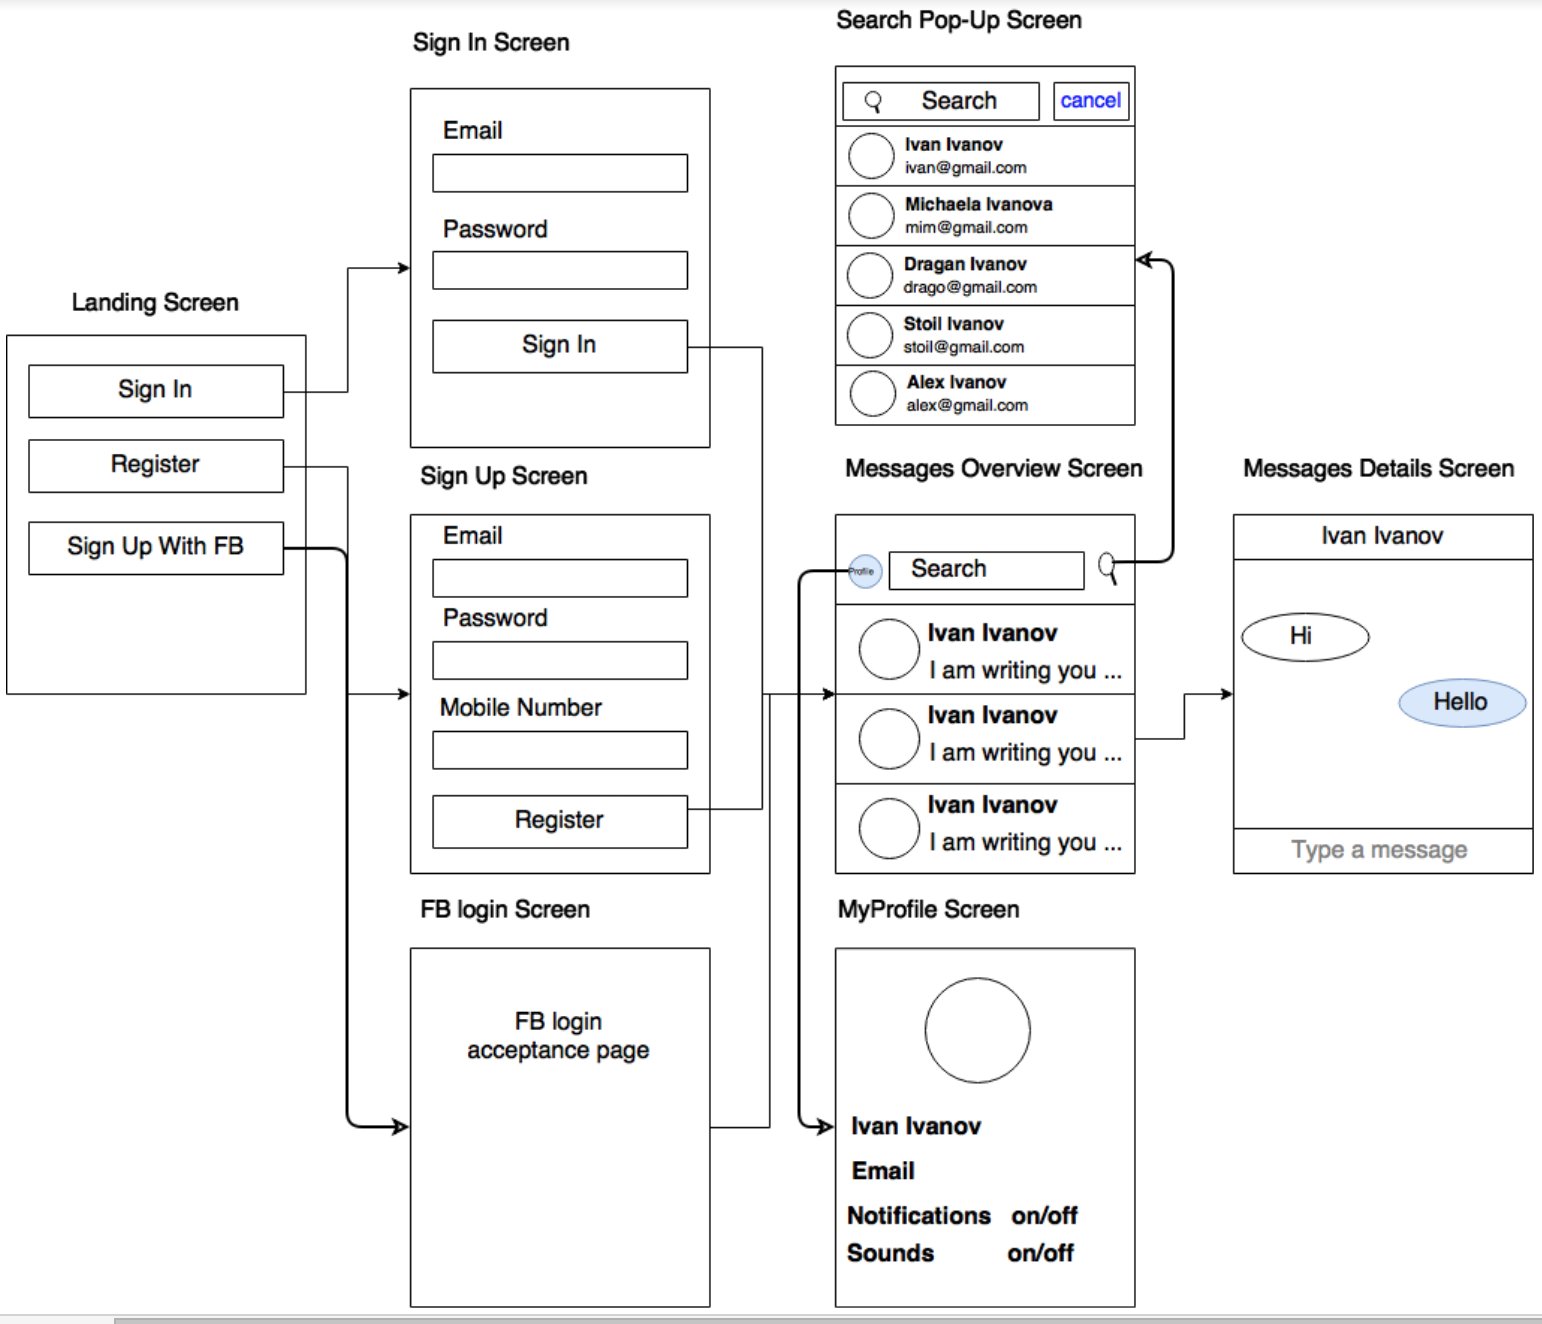
\includegraphics[width=1\textwidth, hsize=0.8\hsize]{Design.png}
\caption{Project Aloha prototype}
\label{fig:figgantt}
\end{figure}

In order to start a communication, client iOS/web either starts from previous chat box or searches the name in search box to communicate with one and more than one users by selecting the tick boxes for multiple users for group chat (Messages Overview screen) and then by clicking the chat button will take to another screen (Messages Detailed screen).). Second user will get the instant notification of chat and can reply in Messages Detailed screen, the two users are communicating and might have extra features such as emoticons and photo sharing.\\
\textbf{Strategies:} \\
The aims of the project are divided into a number of modules listed in the Figure 2 "Gantt Chart". The modules are then divided further into sub modules, where each member of the group has been given a task according to their abilities and skills. This enables each member of the group to work independently. For eliminating the burden of documentation on one member and leaving the documentation for last minute each group member is expected to document the task allocated to them. The final report will be added by one member of the group for proofreading and finalizing the structure. The project strategy is to start and finish the project early for avoiding last minute hassles. In order to get a better understanding of the modules implemented, the Table 1 shows the correlation between the high level aims and the technology used to achieve them. \\

\begin{table}[!ht]
\centering
\captionof{table}{Technologies} \label{tab:title} 
\smallskip
\begin{tabular}{l c c}
\hline
& Platform & Technologies used\\[0.5ex]
\hline
&&\\[-2ex]
1 & Server & Python (Linux based System) \\[0.5ex]
\hline
&&\\[-2ex]
2 & Client A (iOS Application) & iOS (implemented in Swift 3.0) \\[0.5ex]
\hline
&&\\[-2ex]
3 & Client B (Website) & JavaScript, CSS and HTML \\[0.5ex]
\hline
&&\\[-2ex]
4 & Database & MySQL \\[0.5ex]
\hline
&&\\[-2ex]
5 & Protocol (Server, Client) & TCP/IP and TSL/SSL \\[0.5ex]
\hline
\end{tabular}
\end{table}

The project will be based on Agile, more specifically SCRUM methodology, as the project would require certain amount of adaptability. For Managing the project, the software Microsoft's "Team Foundation Server" will be used, which gives the ability to create and manage scrum boards This will also help the group to monitor the project,  prioritize requirements and putting them into five sprints which are given in figure 2 "Gantt Chart". \\

\textbf{High Level Work Breakdown structure:}
\begin{table}[!ht] 
\centering
\label{tab:exTable2}
\smallskip
\begin{tabular}{l c }
\hline
High-Level Tasks & No. of days\\[0.5ex]
\hline
Formation of group & 7 \\[0.5ex]
\hline
Introduction, Research, Discussion, suggestions and finalizing basic requirements \\ for the system. & 7 \\[0.5ex]
\hline
Basic interface design and implementation, initial report documentation \\ and presentation. & 7 \\[0.5ex]
\end{tabular}
\end{table}

\begin{table}[!ht] 
\centering
\label{tab:exTable2}
\smallskip
\begin{tabular}{l c }
\hline
Setting up the required tools and technologies (server, Database, Mock server and API \\ Design) and database design and creation. & 3 \\[0.5ex]
\hline
Project aims development, testing and documentation. & 28 \\[0.5ex]
\hline
Final report and presentation. & 4 \\[0.5ex]
\end{tabular}
\end{table}
\textbf{Gantt Chart:}\\
The Gantt chart given below in Figure 2, illustrates group progress and project aims which are divided into sprints. So far the group has worked on the basic design and functionality of the system (communication and sequence diagrams, user experience design flows and TCP Functionality testing).
\begin{figure}[ht!]
\centering
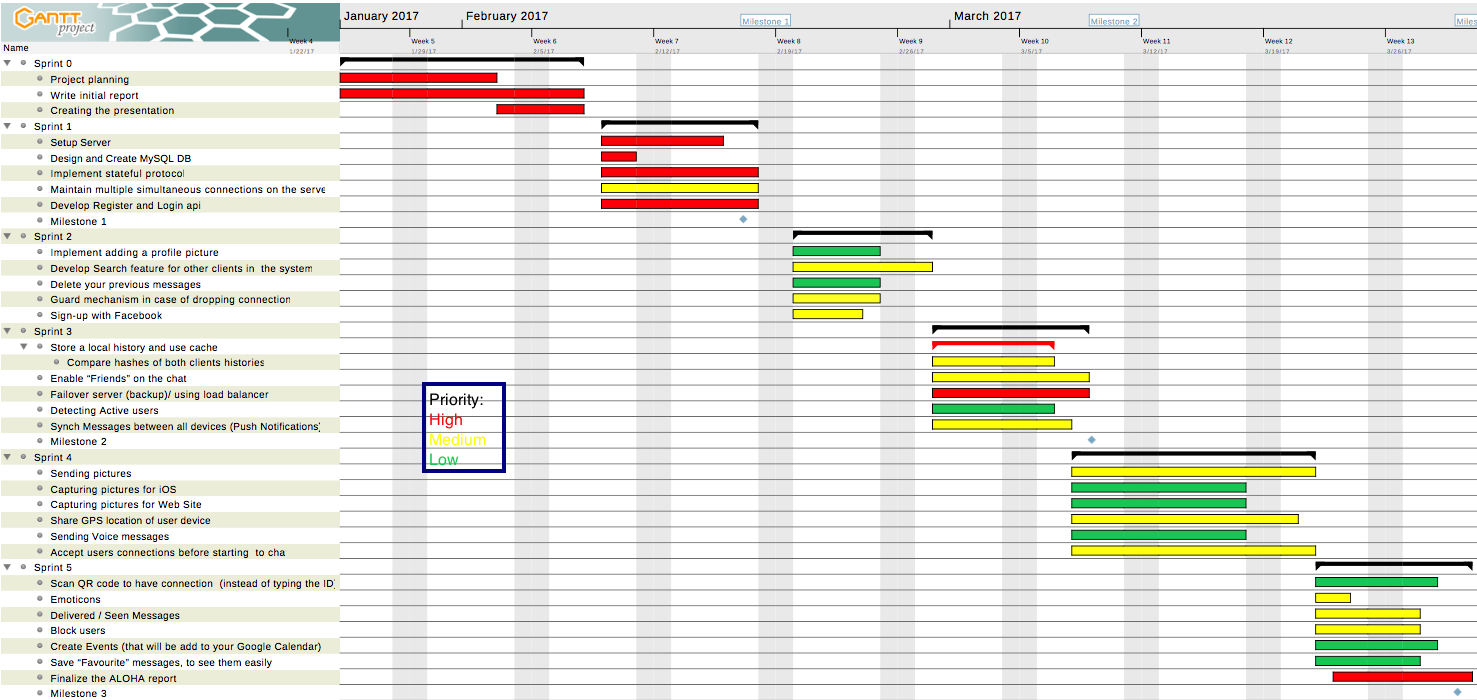
\includegraphics[width=1.1\textwidth]{gant_chart.png}
\caption{Gantt chart}
\label{fig:figgantt}
\end{figure}
\section{Workload Distribution} \label{sec:firstpage}\\
In order to achieve the maximum efficiency for managing the workload, following roles will be distributed among members:\\
\begin{table}[!ht]
\centering
\captionof{table}{Workload Distribution} \label{tab:title} 
\smallskip
\begin{tabular}{l c c}
\hline
Roles & Members\\[0.5ex]
\hline
Project coordinator and  \\ iOS development \\ (Client A) & Lyubomir \\[0.5ex]
\hline
Server(core) & Alex, Darkhan, Sara, Suhrita \\[0.5ex]
\hline
Website (Client B) & Suhrita \\[0.5ex]
\hline
API & Fiza \\[0.5ex]
\end{tabular}
\end{table}

\begin{table}[!ht]
\centering
\smallskip
\begin{tabular}{l c c}
\hline
Database design & All members \\[0.5ex]
\hline
Databases creation & Alex, Lyubomir \\[0.5ex]
\hline
Documentation & All members \\[0.5ex]
\hline
\end{tabular}
\end{table}
\\
\textbf{ Strategies for group collaboration, conflict management and peer evaluation are described here:}

\begin{itemize}
    \item The project will be based on Agile methodology and expects to have a good number of scope changes and eventually will test the product on sprint's (each which will be one week long) avoiding testing the product in the final week.
    \item The group will try to cover the most critical parts of application with unit tests and use a Test Driven Development (TDD) approach to the development process.
    \item The group has set up Google drive to communicate with each other, where files are uploaded online and files can be re-write, if other members come up with better suggestions. 
    \item WhatsApp group has been created for general discussion and instants notifications for the updates. This will keep all the members of the group informed about the project's progress.
    \item Weekly retrospectives - face to face meetings will be held in which the team analyses the results of the previous sprint and based on them every team member shares what he/she thinks the team should:
        \item[--] Start doing / Stop doing / Continue doing
    \item It is necessary for all members to attend face to face weekly meetings. If for some reason a member is unable to attend the meeting then the meeting's updates will be uploaded on the Google drive to keep it informed.  
    \item Decisions will only be taken if there is consensus among members, this will stop one person dominating the group.
    \item In case of a conflict a mediator will be appointed by other group members for resolving the conflict.
    \item A Peer evaluation form will be filled by all members at the end of the project.
    \item Every member will receive an equal number of points(100 divided by 6, gives 16.6), given that no extreme irregularities have been found in the upper mentioned form
\end{itemize}

\textbf{Limitations:}
\begin{itemize}
\item Sever can handle 5000 simultaneous requests 
\item Only English version of application is available
\item HTML5 is needed for supporting web sockets in web client
\item Maximum members a group can have: 10
\end{itemize}

\textbf{Conclusion:}\\
In nutshell, to develop the ALOHA chat project, the upper mentioned tools and strategies will be used to implement a flexible flat design which will be developed sprint by sprint. The overall team's perception of success is creating a MVP (minimum Viable Product) with the basic functions expressed in the UX flowchart, in order to get a customer’s validation.

\end{document}
